\chapter{实验结果及分析}

\section{评价指标}

如3.1节所述,本文使用主要使用最新的SParC数据集作为性能指标。我们使用预测的和标注的SQL语句间的“完全集合匹配精确度”。为避免不影响SQL语义的顺序问题,跟随 [3]中的做法,我们并不使用简单的字符串匹配方法,而是将SQL分解为多个子句,并对每个子句分别按照语义进行忽略顺序的“集合匹配”。本文主要报告两种指标:问题准确率,按照SQL语句统计,对所有交互中的每个SQL语句分别判断是否匹配;交互准确率,按交互统计,仅整个交互中所有查询均匹配才将该交互计算为匹配。

\section{基线方法}

目前SParC数据集上的工作较少。本文主要与EditSQL进行比较,这是截至2020年5月20日已发布论文的模型中效果最好的。与所有提交的模型相比,其排名也很靠前。本文使用了与其相同的解码器算法,但在其他诸多方面做出了改进。EditSQL在编码器方面,使用了多层的LSTM。为了解决跨领域问题,它设计了较为复杂的自然语言和数据库架构间的交叉注意力机制。另外,它使用了独立的交互编码器和交互注意力机制来处理自然语言上下文的问题。

此外,本文也与SParC\cite{sparc19}中发布的两个基线模型进行比较:上下文相关的序列到序列模型 (Context-dependent Seq2Seq) ,它在原始的为ATIS数据集开发的模型基础上新增了使用Bi-LSTM编码数据库架构的能力,和解码未在训练中见过的数据库架构的能力,以适应跨领域的任务。以及SyntaxSQL-con模型,它在原始的为Spider数据集开发的SyntaxSQL\cite{yu-etal-2018-syntaxsqlnet}模型的基础上增加了Bi-LSTM编码交互历史记录的能力,以适应多轮交互的任务。

\section{实现细节}

本文的模型使用PyTorch\cite{pytorch19}实现。在预训练模型上,由于资源限制,本文仅使用了BERT-base或XLNet-base模型。跟随EditSQL的做法,所有LSTM层的隐藏层的维度为300,编码器的LSTM使用1层,解码器的LSTM则使用2层。本文使用了Adam\cite{Adam14}优化器来优化解码的标记的概率分布上的交叉熵损失函数。对于预训练的模型部分,我们使用1e-5的恒定学习率,其他的模型参数初始学习率定为$1e^{-3}$。在5个epoch后,每个epoch学习率递减到上个epoch的0.85。非预训练的参数使用均匀分布$U\left[-0.1,0.1\right]$初始化,除了关系编码使用的参数,它们初始化为0以避免对预训练模型的干扰。训练在模型连续10个epoch未能提升准确率后停止。通常训练在20个epoch左右收敛。

\section{总体结果}

\begin{table}[]
    \centering
    \caption{SParC实验总体结果}
    \begin{tabular}{lrr}
    \hline
                        & 问题准确率 & 交互准确率 \\ \hline
    SyntaxSQL-con       & 18.5  & 4.3   \\
    CD-Seq2Seq          & 21.9  & 8.1   \\
    EditSQL with   BERT & 47.2  & 29.5  \\
    本文模型 with BERT      & 54.3  & 34.6  \\
    本文模型 with XLNet     & 58.5  & 39.6  \\ \hline
    \multicolumn{3}{l}{使用标注的历史SQL查询}    \\ \hline
    EditSQL with   BERT & 53.4  & 29.2  \\
    本文模型 with BERT      & 60.7  & 34.6  \\
    本文模型 with XLNet     & 64.3  & 39.3  \\ \hline
    \end{tabular}
    \label{overall-results}
\end{table}

表\ref{overall-results}展示了本文在SParC数据集上的结果。本文的方法不仅大幅超过了基线模型SyntaxSQL-con和CD-Seq2Seq,而且还显著优于更为复杂的EditSQL模型,达到了58.5\%的问题准确率和39.6\%的交互准确率,分别比EditSQL提升了11.3\%和10.1\%。这归功于本文中的各项改进,包括上下文编码机制、关系编码机制、新的SQL预处理与后处理,以及更新的预训练模型,后文将具体分析。

为了更公平地与基线方法比较,本文也报告了基于BERT模型的结果。但使用更新的XLNet预训练模型有以下好处:1. XLNet使用更大的预料库,其预训练方法也有较大不同,它或许能生成更好的向量表示;2. BERT由于使用预训练的位置嵌入,其位置嵌入最大值为512,将无法完整容纳较大的数据库架构。之前的工作通过将数据库架构在批维度拆分以解决该问题。本文放弃对数据库架构部分使用位置嵌入,转而完全依赖关系编码机制,从而绕过了这个限制,使得BERT的表现略有提升。而XLNet对输入序列的长度没有限制,所以没有类似的问题。从最终结果看,XLNet也取得了更佳的结果。

\begin{figure}[]
    \centering
    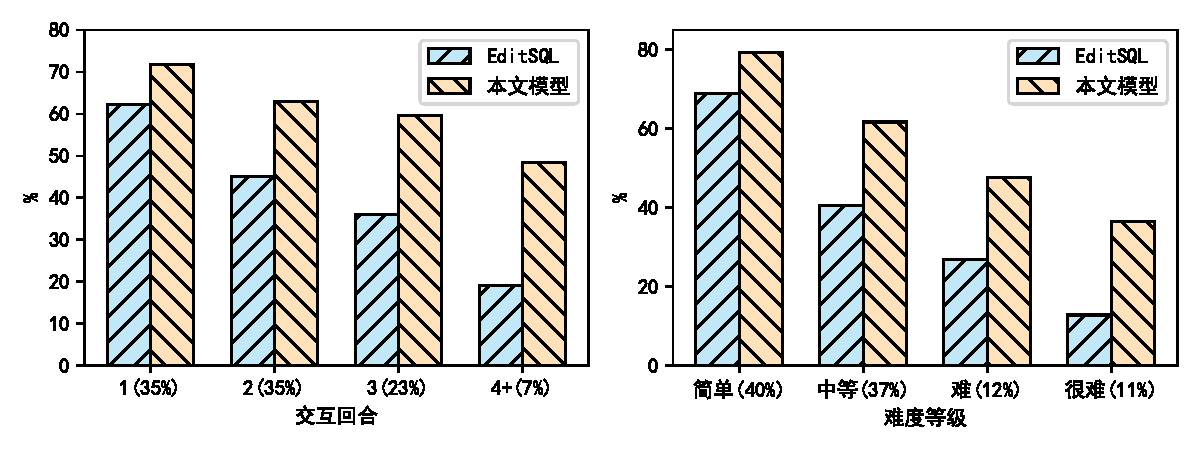
\includegraphics[width=\linewidth]{figure/overall.pdf}
    \caption{SParC实验结果按照交互回合和难度细分。EditSQL使用BERT版本,本文的模型使用XLNet的版本。}
    \label{result-subdivide}
\end{figure}

为了更好地了解模型在用户交互过程中的表现,图\ref{result-subdivide}(左)展示了按照交互轮数细分的指标。随着交互轮数的增加,预测出正确的SQL语句将越来越困难,这是因为自然语言上下文的增长,以及SQL语句本身的复杂度的增加。本文的方法大幅提升了在交互回合数较多时的准确率,特别地,在第四或更多回合时,本文将准确率从19.1\%提升至了48.4\%。类似地,图\ref{result-subdivide}(右)展示了按照难度等级细分的指标。本文的模型在更难的语句中取得的提升更加明显。

\section{消融实验}

\subsection{SQL预处理与后处理效果}

本文进一步研究了SQL预处理和后处理对实验效果的影响。由于SQL具有严格的语法,预处理可操作的范围较广。但本文的研究集中在FROM子句中,因为通常FROM子句是繁琐重复的。

EditSQL也进行了SQL预处理,但没有对此进行讨论。EditSQL的预处理方案是简单地去除整个FROM子句,该方案后文称为“无FROM”。这样的预处理方案虽然能有效提升效果,但有很明显的不足之处:FROM子句中的信息并非都是可以还原的,使用“无FROM”方案预处理过后,将有17.3\%的语句无法通过配套的后处理还原。

本文使用的方案称为“FROM未引用表”,该方案则有效地缓解了这一问题,通过在FROM子句中依然保留一些最有价值的信息,使得仅有2.3\%的语句无法在后处理中还原,余下的无法还原的原因包括:数据集中标注的外键不完整,同一个表参与JOIN多次,使用多个键进行的JOIN等。这些问题难以在当前预处理框架中解决。

同时,本文还对比了一些其他预处理方案:
\begin{itemize}
    \item FROM所有表:简单的在FROM子句中去除所有JOIN,保留所有表名。
    \item FROM未在SELECT中引用的表:类似于“FROM未引用表”,但保留所有未在SELECT子句中引用的表。
    \item SELECT提示:去除整个FROM子句,但将未在SQL其他部分引用的表以特殊标记的形式添加到SELECT子句中。
\end{itemize}

\begin{figure}[]
    \centering
    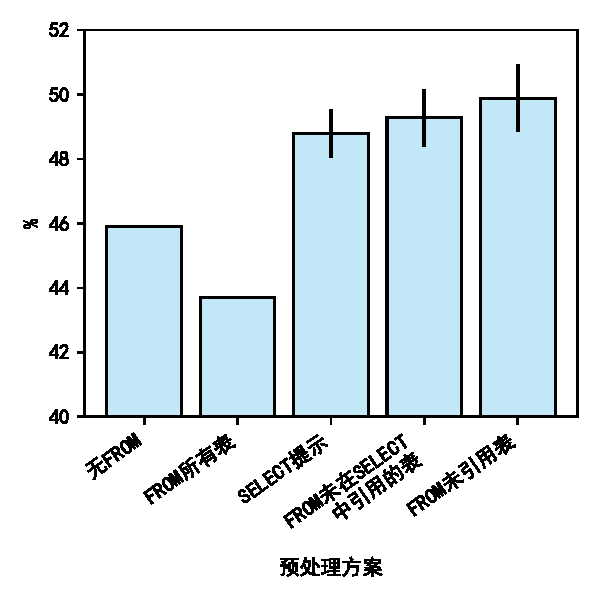
\includegraphics{figure/preprocess.pdf}
    \caption{各种预处理方案对比。在EditSQL的基础上实验不同的预处理方案。图中误差线展示了基于7次实验估计的95\%置信区间}
    \label{preprocess-results}
\end{figure}

图\ref{preprocess-results}展示了各种方案的实验结果。从结果中可以看到,本文使用的“FROM未引用表”效果最佳,而“FROM所有表”方案的效果最差,甚至低于“无FROM”方案。可见,虽然“无FROM”方案有明显丢失信息的问题,但它对提升该任务的效果依然是有积极意义的。对比“FROM所有表”,“FROM未在SELECT中引用的表”和“FROM未引用表”三个方案,其包含的冗余信息依次减少,效果依次上升,这可以解释为网络并不能很好地理解这些信息是冗余的,当要处理的信息越多时,网络出错的概率也就越高。

\subsection{上下文编码机制效果}

\begin{figure}[]
    \centering
    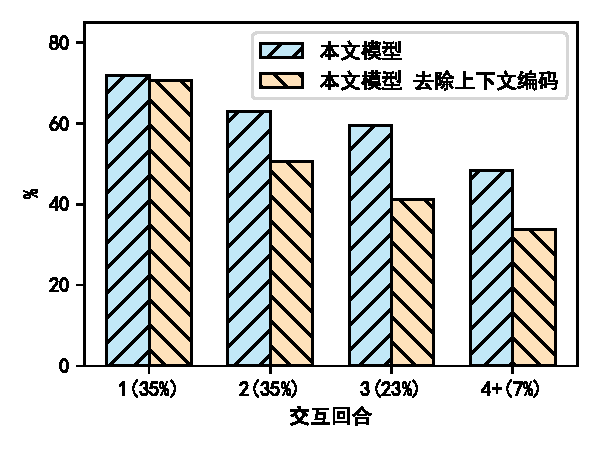
\includegraphics{figure/prefix.pdf}
    \caption{上下文编码消融实验结果,按交互回合细分}
    \label{context-results}
\end{figure}

本文对上下文编码机制的效果进行了消融实验,表\ref{ablation-results}展示了实验结果。此外,将本文提出的上下文编码机制和EditSQL中使用的“交互编码器”进行对比,并将指标按照交互轮数细分展示,如图\ref{context-results}所示。上下文编码机制能帮助网络更好地理解自然语言的上下文信息。整体上,上下文编码机制使准确率提升了4.3\%。其提高在于第二回合及以后的交互中,也就是所有需要处理上下文信息的回合。

\subsection{关系编码机制效果}

\begin{table}[]
    \centering
    \caption{消融实验结果}
    \begin{tabular}{lrr}
    \hline
            & 问题准确率 & 交互准确率 \\ \hline
    本文模型    & 58.5  & 39.6  \\
    - 上下文编码 & 54.2  & 33.9  \\
    - 关系编码  & 57.1  & 38.9  \\ \hline
    \end{tabular}
    \label{ablation-results}
\end{table}

本文也对关系编码机制的效果进行了消融实验。表\ref{ablation-results}中展示了是否使用关系编码机制的效果对比,结果显示关系编码机制能使效果有小幅提升。RAT-SQL\cite{ratsql19}中也报告了类似的机制,在它们的实验中,关系编码带来的提升很大,而本文的提升幅度有限。本文推测原因可能是,在预训练的网络中,网络已经足够强,而能通过内容自行归纳出一些关系,使得额外编码的关系提升有限。另一可能的解释为,由于已经进行了预训练,网络不能充分利用新编码的关系。

\section{错误分析}

\begin{figure}[]
    \centering
    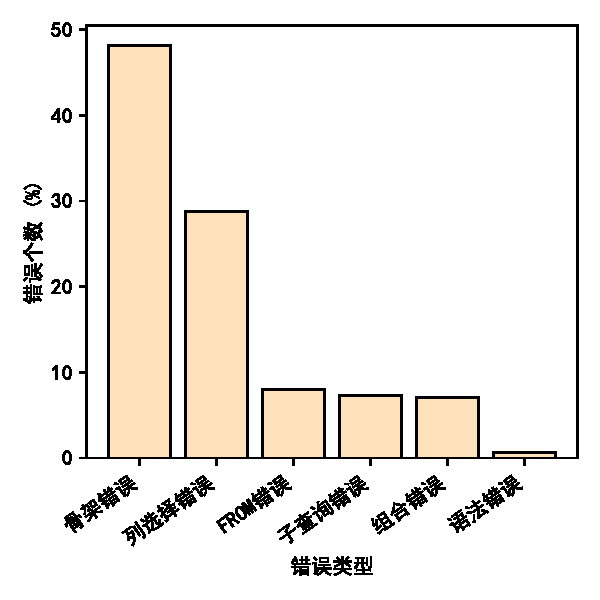
\includegraphics{figure/error.pdf}
    \caption{预测错误分析}
    \label{error}
\end{figure}

本文对模型预测错误的语句进行了分析,具体方法是将预测的SQL语句和标注的SQL语句分别转换成抽象语法树,并对语句的各个部分进行对比,结果如图\ref{error}所示。尽管在解码时没有使用SQL的语法进行约束,解码的结果只有很少量的语法错误,其中大多数是括号不匹配等错误。这可能说明模型对SQL的语法已经能较好地掌握了。对于包含组合和子查询的复杂语句模型还较难处理,模型仅正确预测出了39个组合结构中的7个(18\%),和75子查询结构中的42个(56\%)。鉴于巨大的搜索空间和很少的训练数据,这是可以理解的。但测试数据较少,所以这类错误总量也较少。绝大多数错误都来自单个子查询内的错误。其中较高层次的骨架错误和较低层次的列选择错误都有较高的比例,这意味着对于未来的研究来说,各个层次都是很重要的。由于本文特别对FROM子句部分进行了预处理,所以也特别分析了FROM子句的错误情况。在经过预处理之后,相对来说,FROM子句造成的错误是比较少的。

\section{本章小结}

本章中介绍了本文提出的模型在SParC数据集上的实验结果,得益于本文提出的各项改进,本文的效果显著超过了目前在该任务上的最佳模型。本章还对本文提出的各种改进进行了消融实验,验证的它们各自的效果。本章还对模型的错误进行了分析,这将帮助未来的工作确定方向。
